\section{Architecture}

\subsubsection{Core Architecture}

The core of Apache ActiveMQ Artemis is a simple set of Plain Old Java Objects (POJOs). It is designed in a way to use as few external dependencies as possible. The makes Apache ActiveMQ Artemis to be embedded in any project or injected via dependency injection.

Apache ActiveMQ Artemis comes with its own extreme high-performance journal which is used for message and other persistence. This persistent journal allows Apache ActiveMQ Artemis to get high performance that just cannot be obtained by the utilization of a relational database for persistence.

Apache ActiveMQ Artemis currently offers two APIs for the client side that can be used for messaging.

\begin{itemize}
    \item \textbf{Core client API:}
          An API that allows clients to use complete functionality of messaging without few of the complexities of JMS.

    \item \textbf{JMS client API:}
          This is a standard JMS API for the client.

\end{itemize}

\makeatletter
\setlength{\intextsep}{20pt}
\makeatother

\begin{figure}[h!]
\centering
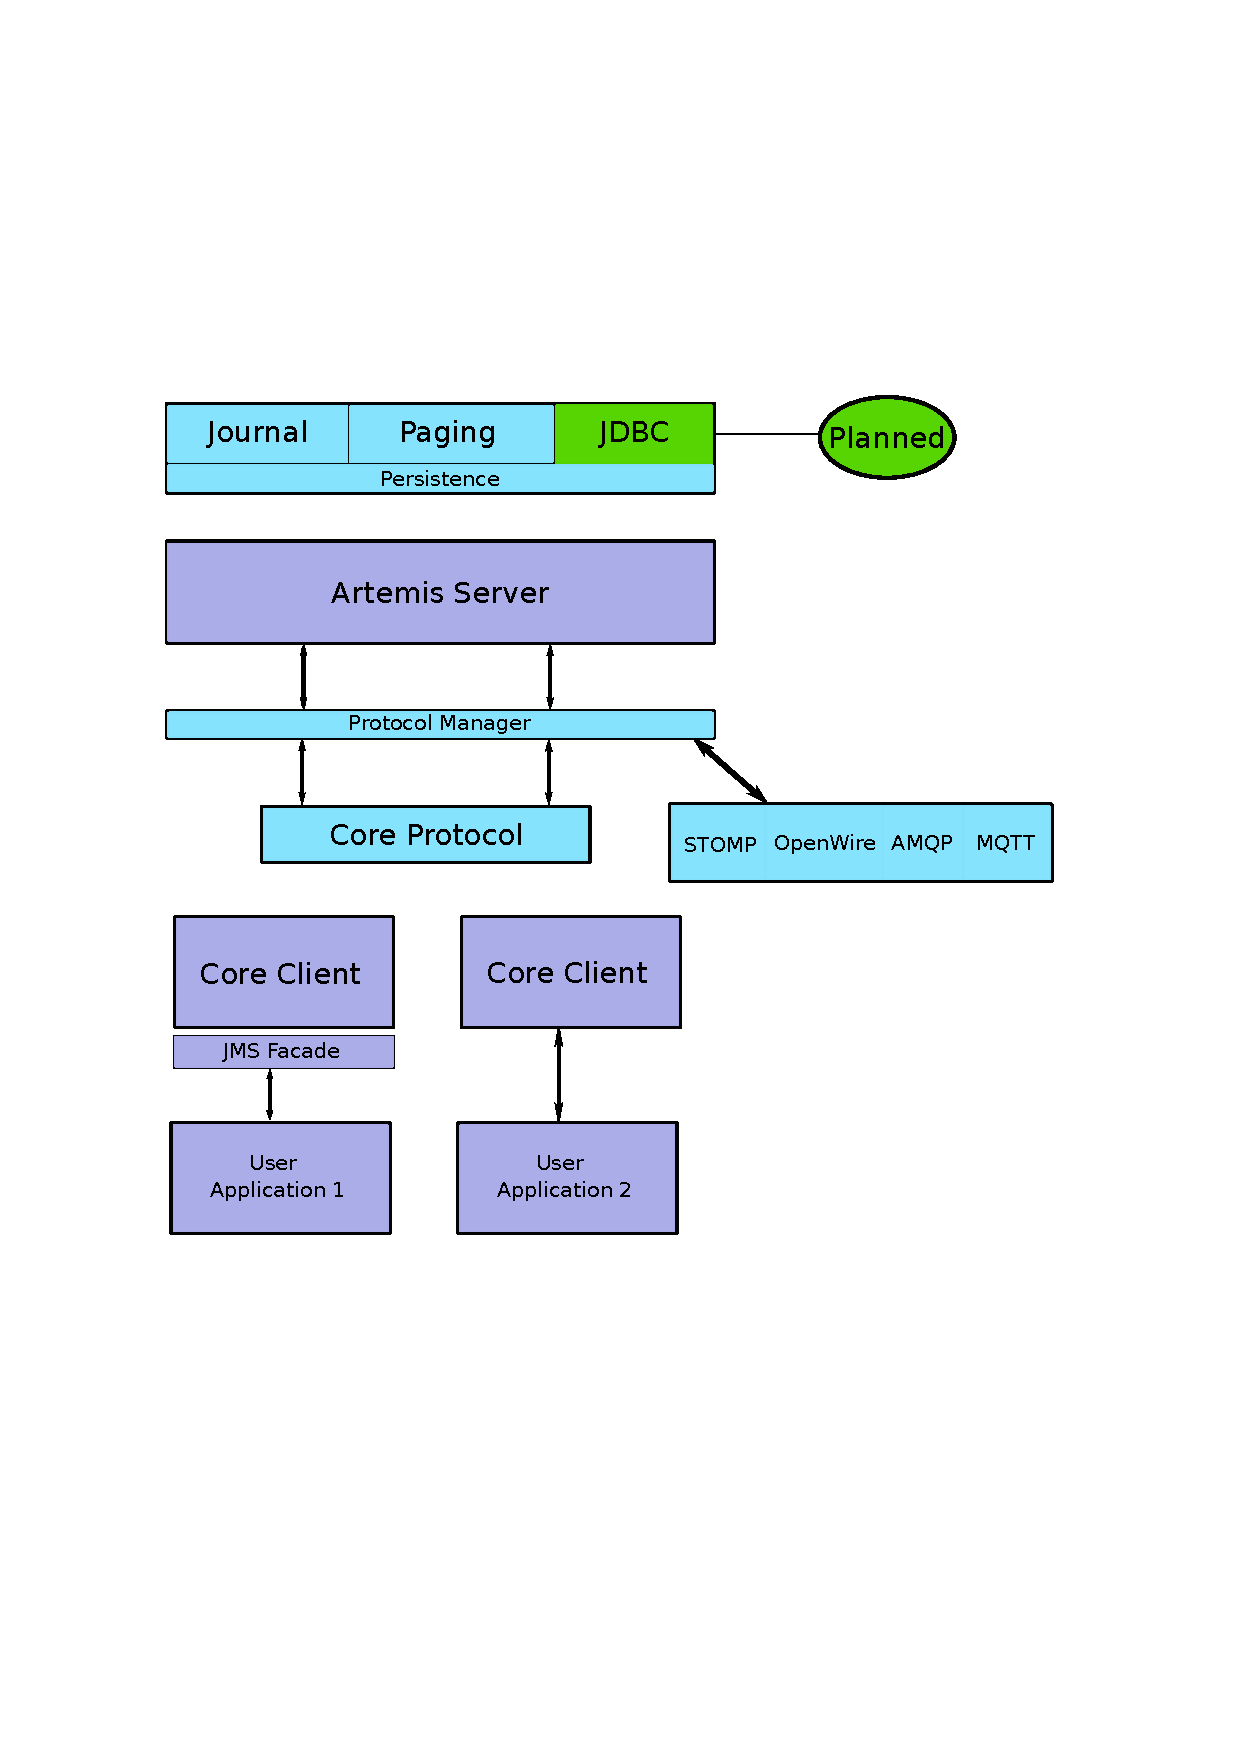
\includegraphics[keepaspectratio, width=.9\textwidth]{artemis.pdf}
\caption{Apache ActiveMQ Artemis High Level Architecture}\label{figures:artemis}
\end{figure}

Apache ActiveMQ Artemis supports protocols such as OpenWire, STOMP, AMQP, and MQTT. Apart from these, a client can choose to communicate using JMS as well via the core protocol. Apache ActiveMQ Artemis is protocol agnostic and hence it does not understand JMS. When the client uses the JMS API, the JMS interactions are translated to the core API using the wire format of the Apache ActiveMQ Artemis. On the client side, a JMS facade layer is used to implement JMS semantics.

Figure \ref{figures:artemis} shows the high level architecture of Apache ActiveMQ Artemis. It also shows the interaction of two applications. One application interacts using the JMS client API and another application uses the core client API for communication with the server. A facade layer can be seen for the application that uses the JMS client API for interaction.